\documentclass{article}

\usepackage[utf8]{inputenc}
\usepackage[ngerman]{babel}
\usepackage{amsmath}
\usepackage{url}
\usepackage[pdftex]{graphicx}
 
\title{Object Caching\\Project Proposal}
\author{Lukas Hofmaier, Raphael Kohler, Timon Brüllmann}
\date{\today}
\begin{document}
\maketitle
\section{Betreuer}
J.M.Joller  Abteilung für Informatik HSR/FHO

\section{Ausgangslage}
Grosse Applikationen sind heute häufig über mehrerer Rechner verteilt, für die Kommunikation zwischen den beteiligten Rechnern wird heutzutage meist die Remote Procedure Call (RPC) Technik verwendet. Sie ermöglicht den Aufruf von Funktionen in anderen Adressräumen. Java bietet bereits eine eingebaute RPC- Mechanismus an, der unter dem Namen Remote Method Invocation (RMI) bekannt ist. 
Das Hauptproblem dieser Technik liegt in der hohen Latenz zwischen dem absetzen des Befehls und dem Empfang des Resultats. Immer wenn eine Methoden auf einem Objekt aufgerufen wird, welches nicht im selben Adressraum gespeichert ist, tritt diese Verzögerung auf.
Applikationen werden heute meist auf Basis des Client- Server Konzept aufgebaut. Wird die Kommunikation zwischen den Clients und dem Server mit einer RPC Technik implementiert,  wird der Server zwangsläufig zum  Flaschenhals für das gesamte System, da alle Objekte auf dem Server lagern und somit alle RPC auf dem Server ausgeführt werden müssen.\\
In dieser Semesterarbeit soll nun eine Lösung erarbeitet werden, welche die gesamt Performance eines verteilten Software Systems steigert ohne dass die Konsistenz der Daten negative beeinträchtigt wird.
\section{Technologische Rahmenbedingungen}
Die Lösung wird in Java entwickelt und als externe Datendarstellung wird XML verwendet, diese bietet den grossen Vorteil von einer plattformneutralen Datendarstellung. Jegliche Sicherheitsaspekte sind nicht Thema dieser Semesterarbeit und sollen fürs erste nicht berücksichtigt werden (Zugriffskontrolle).
\section{Ziel der Arbeit}

Als Ausgangslage für das gesamte Projekt wird folgendes Szenario eingesetzt. Es wird ein verteiltes System mit einem Server und zwei Clients verwendet.\\
\begin{center}
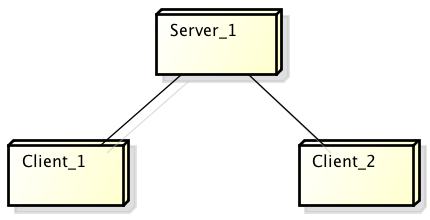
\includegraphics[scale=0.85]{Deployment.png}
\end{center}
Alle Objekte werden auf dem Server instanziiert. Um die Komplexität gering zuhalten wird es nur einen Objekttyp geben. Dadurch wird der Entwicklungsaufwand verringert, welcher für das Management bei zulassen jeglicher Objekttypen bestünde. Der Typ des Objekts wird Account heissen und verfügt über zwei Methoden zur Datenmanipulation. Die eine Methode setzt den neuen Konto-stand und über die zweite Methode kann der aktuelle Kontostand abgefragt werden. In einem ersten Schritt wird es nur ein Objekt auf dem Server instanziiert. Im zweiten Teil der Semesterarbeit werden dann mehrere Account Objekte angelegt.\\
In der ersten Phase wird eine eigene RMI With Coherence Control Lösung implementiert. Die Priorität liegt auf der Erkennung von Konflikten, die Performance kann zu einem späteren Zeitpunkt verbessert werden. Diese Lösung verfügt über keinen Lookup Dienst. Um den Account Typ clientseitig trotzdem zu kennen werden diese fest in die Clients hinein programmiert. Bei dieser Lösung handelt es sich um eine einfache RMI Lösung, welche in der zweiten Phase des Projekts weiter entwickelt wird.
Gleichzeitig wird ein Test Framework entwickelt, dass die verschiedene Lösungsvorschläge, welche im Projektverlauf entwickelt werden, testen kann. Dieses Test System soll Objektkonflikte erfolgreich detektieren, sowie Performancemessungen machen können. Das Test Framework wird so aufgebaut das, es sich von aussen leicht konfigurieren lässt und über Parametervariation verschiedene System-zustände simulieren lassen.\\
\\
In einer zweiten Phase wird die RMI Lösung clientseitig um einen Cache-Mechanismus erweitert. Objekte werden bei dieser Weiterentwicklung clientseitig zwischen gespeichert. Methodenaufrufe die nur lesen werden nun direkt auf dem Client ausgeführt, schreib Operation werden in diese Lösung wiederum auf dem Server abgearbeitet. Die Unterscheidung von Lese und Schreib- Methoden muss durch den User gemacht werden. Des weiteren muss ein Protokoll entwickelt werden, welches effizient die Objekte die sich im Cache befinden invalidiert kann, wenn sich das entsprechende Objekte auf dem Server verändert hat. Diese Lösung wird dann wiederum mit dem Test Framework getestet und mit den Resultaten der ersten Lösung verglichen.\\
Ein weiteres, längerfristiges Ziel ist die Optimierung des Coherence Control Mechanismus sowie eine weiterführende Optimierung des Caches und der damit verbunden Komponenten.

\section{Zur Ausführung}
Die erfolgreiche Bearbeitung dieser Aufgabe setzt Grundkenntnisse in der Programmierung verteilter Systeme voraus (praktische Beispiele, nicht bloss Literaturkenntnisse) sowie die Bereitschaft sich in neue und neuste Ergebnisse einzuarbeiten.
Mit dem Betreuer finden in der Regel wöchentliche Besprechungen statt. Zusätzliche Besprechungen sind nach Bedarf durch die Studierenden zu veranlassen. Das Sitzungsintervall ist flexibel: falls wenig oder keine Probleme auftreten können die Sitzungsintervalle vergrössert werden; falls Probleme auftauchen, werden die Intervalle verkleinert.\\
Alle Besprechungen sind von den Studenten mit einer Traktandenliste vorzubereiten und die Ergebnisse sind in einem Protokoll zu dokumentieren, das dem Betreuer per E-Mail zugestellt wird.\\
Für die Durchführung der Arbeit ist ein Projektplan zu erstellen. Dabei ist auf einen kontinuierlichen und sichtbaren Arbeitsfortschritt zu achten. An Meilensteinen gemäss Projektplan sind einzelne Arbeitsresultate in vorläufigen Versionen abzugeben. 
\section{Dokumentation und Abgabe}
Wegen der beabsichtigten Verwendung der Ergebnisse in weiteren Projekten wird auf Vollständigkeit sowie (sprachliche und grafische) Qualität der Dokumentation erhöhter Wert gelegt.\\
Die Dokumentation zur Projekt- Planung und –Verfolgung ist gemäss den Richtlinien der Abteilung Informatik anzufertigen. Die Detailanforderungen an die Dokumentation der Recherche- und Ent-wicklungsergebnisse werden entsprechend dem konkreten Arbeitsplan festgelegt.\\
Die Dokumentation ist vollständig auf CD abzugeben oder Zugriff auf eine Ablage (SVN, GIT).
Neben der Dokumentation sind abzugeben:
\begin{itemize}
\item alle zum Nachvollziehen der Arbeit notwendigen Ergebnisse und Daten (Quellcode, Buildskripte, Testcode, Testdaten usw.)
\item Material für eine Abschlusspräsentation (ca. 20’)
\end{itemize}

\section{Termine}

\begin{tabular}{l|ll}
Woche & Tasks \\ \hline
1 & Beginn der Studienarbeit; Kick-off Meeting bei Staila im Technopark \\
4 & Abgabe Project Proposal\\
5 & Phase 1 beendet; Test Framework sowie die „RMI with Coherence Control“ Lösung fertig.\\
12 &  Phase 2 beendet. „RMI with Cache“ fertig und getestet. \\
13 & Auswertung der Test Resultate
\end{tabular}

\section{Literaturhinweise}
Generelle Referenzen:\\
Siehe Vorlesung über Verteilte Software Systeme.\\
Weitere Literatur wird bei Bedarf zur Verfügung gestellt!
\section{Beurteilung}
Eine erfolgreiche Studienarbeit erhält 8 ECTS-Punkten (1 ECTS Punkt entspricht einer Arbeitsleistung von ca. 25 bis 30 Stunden). Für die Modulbeschreibung der Studienarbeit siehe 
\url{https://unterricht.hsr.ch/staticWeb/allModules/10938_M_SAI.html}.\\ \\
\begin{tabular}{l p{3cm} l l l}
Gesichtspunkt & Gewicht \\ \hline
1. Organisation, Durchführung & 1/5 \\
2. Berichte (Abstract, Management Summary, techn. u. persönliche Berichte) sowie Gliederung, Darstellung, Sprache der gesamten Dokumentation & 1/5 \\
3. Inhalt*) & 3/5
\end{tabular}
*) Die Unterteilung und Gewichtung von 3. Inhalt wird im Laufe dieser Arbeit mit dem Studenten vereinbart. Im Übrigen gelten die Bestimmungen der Abt. Informatik zur Durchführung von Studienarbeiten.\\ \\
Rapperswil, den\\
Der verantwortliche Dozent\\
\end{document}